\documentclass[fleqn, a4paper, 12pt, twoside]{article}

\newcounter{recitationcount} %creates a new counter for recitation numbers (must be executed before exsheets is loaded)
\newcommand\recitation{\refstepcounter{recitationcount}}

\usepackage[counter-within = recitationcount]{exsheets}
\usepackage{tasks}
\usepackage{amsmath, amssymb, amsthm} %standard AMS packages
\usepackage{marginnote} %marginnotes
\usepackage{gensymb} %miscellaneous symbols
\usepackage{commath} %differential symbols
\usepackage{xcolor} %colours
\usepackage{cancel} %cancelling terms
\usepackage{siunitx} %formatting units
\usepackage{tikz, pgfplots} %diagrams
	\usetikzlibrary{calc, hobby, patterns, intersections}
\usepackage{graphicx} %inserting graphics
\usepackage{hyperref} %hyperlinks
\usepackage{datetime} %date and time
\usepackage{ulem} %underline for \emph{}
\usepackage{xfrac} %inline fractions
\usepackage{enumerate} %numbered lists
\usepackage{float} %inserting floats
\usepackage{circuitikz} %circuit diagrams

\newcommand\numberthis{\addtocounter{equation}{1}\tag{\theequation}} %adds numbers to specific equations in non-numbered list of equations

\newcommand{\AxisRotator}[1][rotate=0]{
	\tikz [x=0.25cm,y=0.60cm,line width=.2ex,-stealth,#1] \draw (0,0) arc (-150:150:1 and 1);%
} %rotation symbols on axes

\theoremstyle{definition}
\newtheorem{example}{Example}
\newtheorem{definition}{Definition}

\theoremstyle{theorem}
\newtheorem{theorem}{Theorem}

\newcommand{\curl}{\mathrm{curl\,}}

\makeatletter
\@addtoreset{section}{part} %resets section numbers in new part
\makeatother

\newcommand\blfootnote[1]{%
	\begingroup
	\renewcommand\thefootnote{}\footnote{#1}%
	\addtocounter{footnote}{-1}%
	\endgroup
}

\RenewQuSolPair{question}[name=Recitation \therecitationcount\ -- Exercise]{solution}[name=Recitation \therecitationcount\ -- Solution]

\SetupExSheets{solution/print = true, totoc = true} %prints all solutions by default

%opening
\title{Physics 2 : Recitations}
\author{Aakash Jog}
\date{2014-15}

\begin{document}

\maketitle
%\setlength{\mathindent}{0pt}

\blfootnote
{	
	\begin{figure}[H]
		\includegraphics[height = 12pt]{cc.eps}
		\includegraphics[height = 12pt]{by.eps}
		\includegraphics[height = 12pt]{nc.eps}
		\includegraphics[height = 12pt]{sa.eps}
	\end{figure}
	This work is licensed under the Creative Commons Attribution-NonCommercial-ShareAlike 4.0 International License. To view a copy of this license, visit \url{http://creativecommons.org/licenses/by-nc-sa/4.0/}.
} %CC-BY-NC-SA licencse

\tableofcontents

\newpage
\section{Instructor Information}

\textbf{Dr. Richard Spitzberg}\\
~\\
Office: Ma Aabadot 119\\
E-mail: rms9999@gmail.com\\

\newpage

\part{Electrostatics}

\section{Gravitation and Electromagnetism}

\begin{tabular}{l l}
	Gravitation & Electromagnetism\\
		$F_G = G \dfrac{m_1 m_2}{r^2}$ & $F_E = k \dfrac{q_1 q_2}{r^2}$\\
		$G = 6.7 \times 10^{11} \si{\newton\metre\squared\per\kg\squared}$ & $8.99 \times 10^9 \si{\newton\metre\squared\per\coulomb\squared}$\\
\end{tabular}

\section{Coulomb's Law}

\recitation

\begin{question}
	Four identical charges $q$ are placed in the corners of a square of length $a$. A fifth charge $Q$ is free to move along the straight line perpendicular to the square plane and passing through its centre. When the charge $Q$ is in the same plane as the other charges, all the forces in the system cancel out.
	\begin{enumerate}
		\item Calculate $Q$ for a given $q$ and $a$.
		\item Find the force $\overrightarrow{F(z)}$ acting on the charge $Q$ when it is at height $z$ above the square.
	\end{enumerate}
\end{question}

\begin{solution}[print]
	\begin{figure}[H]
		\begin{tikzpicture}
			\def\a{4};
			
			\draw (-\a/2,-\a/2) rectangle (\a/2,\a/2);
			
			\filldraw ({-\a/2},{-\a/2}) circle [radius = 2pt] node [below left] {$q$};
			\filldraw ({-\a/2},{\a/2}) circle [radius = 2pt] node [above left] {$q$};
			\filldraw ({\a/2},{\a/2}) circle [radius = 2pt] node [above right] {$q$};
			\filldraw ({\a/2},{-\a/2}) circle [radius = 2pt] node [below right] {$q$};
			
			\filldraw (0,0) circle [radius = 2pt] node [left] {$Q$};
		\end{tikzpicture}
	\end{figure}
	Consider $q$ on the top right corner of the square. The total force acting on it is 0. Therefore
	\begin{align*}
		0 &= \dfrac{k q^2}{a^2} \cos \dfrac{\pi}{4} + \dfrac{k q^2}{a^2} \cos \dfrac{\pi}{4} + \dfrac{k q^2}{2 a^2} + \dfrac{2 k Q q}{a^2}\\
		\therefore Q &= - \dfrac{1 + 2 \sqrt{2}}{4} q
	\end{align*}
	~\\
	If $Q$ is at a height $z$ from the plane, the distance between each $q$ and $Q$ is
	\begin{align*}
		r &= \sqrt{z^2 + \left( \dfrac{a}{\sqrt{2}} \right)^2}
	\end{align*}
	Therefore the force of each $q$ on $Q$ is $\dfrac{k Q q}{r^2}$.\\
	Due to symmetry, the components of the forces in the $z$ direction will add up, and all other components will cancel out.\\
	Let the angle between the $z$ direction and the line joining $q$ and $Q$ be $\varphi$.\\
	Therefore, the net force is 
	\begin{align*}
		F &= 4 \dfrac{k Q q}{r^2} \cos \varphi\\
		&= 4 \dfrac{k Q q}{r^2} \dfrac{z}{r}\\
		&= 4 \dfrac{k Q q}{z^2 \left( 1 + \dfrac{a^2}{2 z^2} \right)^{\sfrac{3}{2}}}
	\end{align*}
\end{solution}

\begin{question}
	\begin{enumerate}
		\item A wire of length 3 \si{metre} is charged with 2 \si{\coulomb\per\metre}. What is the wire's total charge?
	\end{enumerate}
\end{question}

\begin{solution}[print]
	\begin{align*}
		\lambda &= \dfrac{Q}{L}\\
		\therefore Q &= L \lambda\\
		&= 6 \si{\coulomb}
	\end{align*}
\end{solution}

\begin{question}
	A wire of length $L$ has the following charge distribution: $\lambda = \lambda_0 \cos \dfrac{\pi x}{L}$, where $x$ is the distance from the wire's edge. What is the wire's total charge?
\end{question}

\begin{solution}[print]
	\begin{align*}
		\lambda &= \dod{q}{x}\\
		\therefore \dod{q}{x} &= \lambda_0 \cos \dfrac{\pi x}{L}\\
		\therefore q &= \int\limits_{0}^{L} \lambda_0 \cos \dfrac{\pi x}{L} \dif x\\
		&= 0
	\end{align*}
\end{solution}

\begin{question}
	A hollow sphere of radius $R$ is uniformly charged with a charge $Q$. Calculate the charge distribution on the surface of the sphere.
\end{question}

\begin{solution}[print]
	\begin{align*}
		\sigma &= \dfrac{Q}{A}\\
		&= \dfrac{Q}{4 \pi R^2}
	\end{align*}
\end{solution}

\begin{question}
	A straight thin wire is uniformly charged with distribution $\lambda$. A charge $q$ is positioned at distance $y_1$ beneath the wire and $r$ away form it.
	\begin{enumerate}
		\item Find the force acting on the charge $q$.
		\item Show that when the charge is positioned in front of the centre of the wire the $\hat{y}$ component of the force is cancelled.
		\item Calculate the force an infinite straight wire will exert on the charge $q$.
	\end{enumerate}
\end{question}

\begin{solution}[print]
	\begin{figure}[H]
		\begin{tikzpicture}
			\def\L{3};
			\def\y{2};
			\def\r{2};
			\def\Y{1};
			
			\def\xMAX{\L + \Y + 1};
			\def\yMAX{\r + 1};
			
			\begin{scope}[gray, -stealth]
				\draw (0,0) -- (\xMAX,0) node [right] {$y$};
				\draw (0,0) -- (0,\yMAX) node [above] {$z$};
			\end{scope}
			
			\draw [ultra thick, red] (0,0) -- (\L,0);
			
			\begin{scope}[|-stealth, yshift = -10]
				\draw (\L,0) -- ++(\Y,0) node [below] {$y_1$};
				\draw (0,0) -- (\y,0) node [below] {$y$};
				\draw [yshift = -10] (0,0) -- (\L,0) node [below] {$L$};
			\end{scope}
			
			\filldraw ({\L + \Y}, \r) circle [radius = 2pt] node [left] {$q$};
			
			\begin{scope}[dashed]
				\draw ({\L + \Y},0) -- ({\L + \Y}, \r) node [midway, right] {$r$};
				\draw (\y,0) -- ({\L + \Y}, \r) node [midway, above left] {$R$};
			\end{scope}
		\end{tikzpicture}
	\end{figure}
	Consider an elemental charge $\dif Q$ of length $\dif y$, at distance $y$ as shown. Let the angle between the line joining $\dif Q$ and $q$ and the $y$ direction be $\theta$.
	\begin{align*}
		F_y &= F \cos \theta\\
		F_z &= F \sin \theta\\
	\end{align*}
	Let
	\begin{align*}
		a &= L + y_1\\
		\therefore R &= \sqrt{r^2 + (a - y)^2}
	\end{align*}
	Therefore,
	\begin{align*}
		\cos \theta &= \dfrac{a - y}{R}\\
		\sin \theta &= \dfrac{r}{R}
	\end{align*}
	Therefore,
	\begin{align*}
		F_y &= k q \int\limits_{0}^{L} \dfrac{\lambda \dif y}{R^2} \dfrac{(a - y)}{R}\\
		&= k q \lambda \int\limits_{0}^{L} \dfrac{\dif y (a - y)}{\left( (a - y)^2 + r^2 \right)^{\sfrac{3}{2}}}\\
		&= k q \lambda \left( \dfrac{1}{\sqrt{{y_1}^2 + r^2}} - \dfrac{1}{\sqrt{a^2 + r^2}} \right)
	\end{align*}
	\begin{align*}
		F_z &= k q \int\limits_{0}^{L} \dfrac{\lambda \dif y}{R^2} \dfrac{r}{R}\\
		&= k q \lambda \int\limits_{0}^{L} \dfrac{r \dif y}{\left( (a - y)^2 + r^2 \right)^{\sfrac{3}{2}}}\\
		&= \dfrac{k q \lambda}{r} \left( \dfrac{a}{\sqrt{r^2 + a^2}} - \dfrac{y_1}{\sqrt{r^2 + {y_1}^2}} \right)
	\end{align*}
	~\\
	When the charge is positioned above the centre of the wire,
	\begin{align*}
		y_1 &= -\dfrac{L}{2}\\
		\therefore a &= \dfrac{L}{2}
	\end{align*}
	Therefore,
	\begin{align*}
		F_y &= k q \lambda \left( \dfrac{1}{\sqrt{{y_1}^2 + r^2}} - \dfrac{1}{\sqrt{a^2 + r^2}} \right)\\
		&= k q \lambda \left( \dfrac{1}{\sqrt{{-\dfrac{L}{2}}^2 + r^2}} - \dfrac{1}{\sqrt{{\dfrac{L}{2}}^2 + r^2}} \right)\\
		&= 0
	\end{align*}
	\begin{align*}
		F_z &= \dfrac{k q \lambda}{r} \left( \dfrac{a}{\sqrt{r^2 + a^2}} - \dfrac{y_1}{\sqrt{r^2 + {y_1}^2}} \right)\\
		&= \dfrac{k q \lambda}{r} \left( \dfrac{\dfrac{L}{2}}{\sqrt{r^2 + {\dfrac{L}{2}}^2}} - \dfrac{-\dfrac{L}{2}}{\sqrt{r^2 + {-\dfrac{L}{2}}^2}} \right)\\
		&= \dfrac{k q \lambda}{r} \left( \dfrac{L}{\sqrt{r^2 + {\dfrac{L}{2}}^2}} \right)\\
		&= \dfrac{k q \lambda}{r} \left( \dfrac{1}{\sqrt{\dfrac{1}{4} + \left( \dfrac{r}{L} \right)^2}} \right)
	\end{align*}
	~\\
	If the line is infinite, $L \to \infty$. Therefore
	\begin{align*}
		F_z &= \dfrac{k q \lambda}{r} \left( \dfrac{1}{\sqrt{\dfrac{1}{4} + \left( \dfrac{r}{L} \right)^2}} \right)\\
		&= \dfrac{2 k q \lambda}{r} 
	\end{align*}
\end{solution}

\section{Gauss' Law}

\recitation
\setcounter{question}{1}

\begin{question}
	A ball of radius $a$ is charged with distribution $\rho$ = $\rho_0 \dfrac{r}{a}$. Find the electric field everywhere.
\end{question}

\begin{solution}
	Consider a spherical Gaussian surface of radius $r$.\\
	If $r \leq a$, the charge in the interior of the Gaussian surface is
	\begin{align*}
		q(r) &= \int\limits_{0}^{r} \dfrac{\rho_0 r}{a} \cdot 4 \pi r^2 \dif r\\
		&= \dfrac{\rho_0}{a} \pi r^4
	\end{align*}
	Therefore, by Gauss' Law,
	\begin{align*}
		E \cdot 4 \pi r^2 &= \dfrac{q(r)}{\varepsilon_0}\\
		\therefore E &= \dfrac{\rho_0 \pi r^4}{4 \pi a r^2}\\
		&= \dfrac{\rho_0 r^2}{4 a \varepsilon_0}
	\end{align*}
	If $r \geq a$, the entire ball of charge is in the interior of the Gaussian surface.\\
	Therefore,
	\begin{align*}
		Q &= q(a)\\
		&= \dfrac{\rho_0}{a} \cdot \pi a^4\\
		&= \rho_0 \pi a^3
	\end{align*}
	Therefore, by Gauss' Law,
	\begin{align*}
		E \cdot 4 \pi r^2 &= \dfrac{Q}{\varepsilon_0}\\
		\therefore E &= \dfrac{Q}{4 \pi r^2 \varepsilon_0}\\
		&= \dfrac{\rho_0 a^3}{4 r^2 \varepsilon_0}
	\end{align*}
	~\\
	Therefore,
	\begin{align*}
		E &=
			\begin{cases}
				\dfrac{\rho_0 r^2}{4 a \varepsilon_0} &;\quad r \leq a\\
				\dfrac{\rho_0 a^3}{4 r^2 \varepsilon} &;\quad r \geq a\\
			\end{cases}
	\end{align*}
\end{solution}

\begin{question}
	An infinitely long cylinder of radius $a$ is charged with distribution $\rho = \rho_0 \dfrac{r}{a}$. Find the electric field everywhere.
\end{question}

\begin{solution}
	Consider a infinite cylindrical Gaussian surface with radius $r$.\\
	If $r \leq a$, the charge in the interior of the Gaussian surface is
	\begin{align*}
		q(r) &= \int\limits_{0}^{r} \dfrac{\rho_0 r}{a} \pi r^2 \dif r\\
		&= \dfrac{2 \pi \rho_0 L r^3}{3 a}
	\end{align*}
	Therefore, by Gauss' Law,
	\begin{align*}
		E \cdot 2 \pi r L &= \dfrac{2 \pi \rho_0 L r^3}{3 a \varepsilon_0}\\
		\therefore E &= \dfrac{\rho_0 r^2}{3 a \varepsilon_0}
	\end{align*}
	If $r \geq a$, the entire cylinder of charge is in the interior of the Gaussian surface.\\
	Therefore,
	\begin{align*}
		Q &= q(a)\\
		&= \dfrac{2 \pi \rho_0 L a^3}{3 a}\\
		&= \dfrac{2 \pi \rho_0 L a^2}{3}
	\end{align*}
	Therefore, by Gauss' Law,
	\begin{align*}
		E \cdot 2 \pi r L &= \dfrac{2 \pi \rho_0 L a^2}{3 \varepsilon_0}\\
		\therefore E &= \dfrac{\rho_0 a^2}{3 \varepsilon_0 r}
	\end{align*}
	~\\
	Therefore,
	\begin{align*}
		E &= 
			\begin{cases}
				\dfrac{\rho_0 r^2}{3 a \varepsilon_0} &;\quad r \leq a\\
				\dfrac{\rho_0 a^2}{3 \varepsilon_0 r} &; \quad r \geq a\\
			\end{cases}
	\end{align*}
\end{solution}

\begin{question}
	Find the electric field due to a thin infinite plane of uniform charge distribution $\sigma$.
\end{question}

\begin{solution}
	Consider a cylindrical Gaussian surface, with ends of area $A$, as shown.
	\begin{figure}[H]
		\begin{tikzpicture}
			\def\h{2};
			\def\r{1};
			\def\L{5};
			
			\draw [blue] ({-\L/2},0) -- ({\L/2},0) node [right] {$\sigma$};
			
			\begin{scope}[red]
				\draw (0,{-\h/2}) circle [x radius = \r, y radius = 0.4*\r];
				\draw (0,{\h/2}) circle [x radius = \r, y radius = 0.4*\r];
				
				\draw ({-\r},{-\h/2}) -- ({-\r},{\h/2});
				\draw ({\r},{-\h/2}) -- ({\r},{\h/2});
			\end{scope}
		\end{tikzpicture}
	\end{figure}
	The charge in the interior of the surface is
	\begin{align*}
		\dif q &= A \sigma
	\end{align*}
	Therefore, by Gauss' Law,
	\begin{align*}
		E_1 \cdot A_1 + E_2 \cdot A_2 &= \dfrac{A \sigma}{\varepsilon_0}\\
		\therefore 2 E A &= \dfrac{A \sigma}{\varepsilon_0}\\
		\therefore E &= \dfrac{\sigma}{2 \varepsilon_0}
	\end{align*}
\end{solution}

\recitation

\setcounter{question}{1}

\begin{question}
	A system of four charges is constructed as shown.
	\begin{figure}[H]
		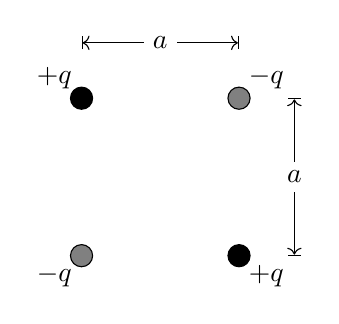
\begin{tikzpicture}
			\def\a{2};
			
			\filldraw [fill = gray]
				({\a/2},{\a/2}) circle (4pt) node [above right] {$-q$}
				({-\a/2},{-\a/2}) circle (4pt) node [below left] {$-q$};
				
			\filldraw [fill = black]
				({-\a/2},{\a/2}) circle (4pt) node [above left] {$+q$}
				({\a/2},{-\a/2}) circle (4pt) node [below right] {$+q$};
				
			\begin{scope}[|<->|]
				\draw [yshift = 20] ({-\a/2},{\a/2}) -- ({\a/2},{\a/2}) node [midway, fill = white] {$a$};
				\draw [xshift = 20] ({\a/2},{-\a/2}) -- ({\a/2},{\a/2}) node [midway, fill = white] {$a$};
			\end{scope}
		\end{tikzpicture}
	\end{figure}
	\begin{tasks}
		\task Calculate the work needed to build this system.
		\task What is the potential in the centre of the system?
		\task Calculate the potential in each of the corners (calculate as if there is no charge in the corner you are calculating for).
	\end{tasks}
\end{question}

\begin{solution}
	\begin{tasks}
		\task
			Let the positions of the charges be A, B, C, D.
			\begin{figure}[H]
				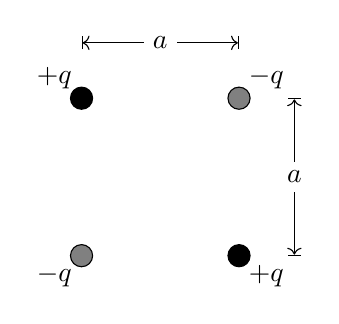
\begin{tikzpicture}
					\def\a{2};
					
					\filldraw [fill = gray]
						({\a/2},{\a/2}) circle (4pt) node [above right] {$-q$}
						({-\a/2},{-\a/2}) circle (4pt) node [below left] {$-q$};
					
					\filldraw [fill = black]
						({-\a/2},{\a/2}) circle (4pt) node [above left] {$+q$}
						({\a/2},{-\a/2}) circle (4pt) node [below right] {$+q$};
					
					\begin{scope}[|<->|]
						\draw [yshift = 20] ({-\a/2},{\a/2}) -- ({\a/2},{\a/2}) node [midway, fill = white] {$a$};
						\draw [xshift = 20] ({\a/2},{-\a/2}) -- ({\a/2},{\a/2}) node [midway, fill = white] {$a$};
					\end{scope}
				\end{tikzpicture}
			\end{figure}
			The work done to bring the first charge from infinity to A is
			\begin{align*}
				W_{\textnormal{A}} &= 0
			\end{align*}
			The work done to bring the first charge from infinity to B is
			\begin{align*}
				W_{\textnormal{B}} &= \dfrac{1}{4 \pi \varepsilon_0} \dfrac{q^2}{a \sqrt{2}}
			\end{align*}
			Similarly for the other two charges.\\
			Therefore,
			\begin{align*}
				W &= 0 + \dfrac{q^2}{4 \sqrt{2} \pi \varepsilon_0} + \dfrac{-2q^2}{4 \pi \varepsilon_0 a} + \left( \dfrac{-2q^2}{4 \pi \varepsilon_0 a} + \dfrac{q^2}{4 \sqrt{2} \pi \varepsilon_0} \right)\\
				&= \dfrac{q^2}{2 \sqrt{2} \pi \varepsilon_0} - \dfrac{q^2}{\pi \varepsilon_0 a}
			\end{align*}
		\task
			\begin{align*}
				V_{\textnormal{centre}} &= V_{q} + V_{q} + V_{-q} + V_{-q}\\
				&= \dfrac{q}{4 \pi \varepsilon_0 \left( \dfrac{a}{\sqrt{2}} \right)} + \dfrac{q}{4 \pi \varepsilon_0 \left( \dfrac{a}{\sqrt{2}} \right)} - \dfrac{q}{4 \pi \varepsilon_0 \left( \dfrac{a}{\sqrt{2}} \right)} - \dfrac{q}{4 \pi \varepsilon_0 \left( \dfrac{a}{\sqrt{2}} \right)}\\
				&= 0
			\end{align*}
		\task
			\begin{align*}
				V_{\textnormal{A}} &= \dfrac{1}{4 \pi \varepsilon_0} \dfrac{-q}{a} + \dfrac{1}{4 \pi \varepsilon_0} \dfrac{-q}{a} + \dfrac{1}{4 \pi \varepsilon_0} \dfrac{q}{\sqrt{2} a}\\
				V_{\textnormal{B}} &= \dfrac{1}{4 \pi \varepsilon_0} \dfrac{-q}{a} + \dfrac{1}{4 \pi \varepsilon_0} \dfrac{-q}{a} + \dfrac{1}{4 \pi \varepsilon_0} \dfrac{q}{\sqrt{2} a}\\
				V_{\textnormal{C}} &= \dfrac{1}{4 \pi \varepsilon_0} \dfrac{q}{a} + \dfrac{1}{4 \pi \varepsilon_0} \dfrac{q}{a} + \dfrac{1}{4 \pi \varepsilon_0} \dfrac{-q}{\sqrt{2} a}\\
				V_{\textnormal{D}} &= \dfrac{1}{4 \pi \varepsilon_0} \dfrac{q}{a} + \dfrac{1}{4 \pi \varepsilon_0} \dfrac{q}{a} + \dfrac{1}{4 \pi \varepsilon_0} \dfrac{-q}{\sqrt{2} a}
			\end{align*}
	\end{tasks}
\end{solution}

\begin{question}
	A ring of radius $R$ is charged with total charge $Q$.
	\begin{tasks}
		\task Calculate the electric field in the centre of the ring.
		\task Calculate the potential in the centre of the ring by integrating the contributions of the infinitesimal charge elements of the ring.
	\end{tasks}
\end{question}

\begin{solution}
	\begin{tasks}
		\task
			Due to the symmetry of the ring, the field due to every elemental charge $\dif q$ will be cancelled out by the field due to a elemental charge diametrically opposite to $\dif q$.\\
			Therefore, 
			\begin{align*}
				\overrightarrow{E} &= 0
			\end{align*}
		\task
			\begin{align*}
				\dif V &= \dfrac{\dif q}{4 \pi \varepsilon_0 R}\\
				\therefore V &= \dfrac{Q}{4 \pi \varepsilon_0 R}
			\end{align*}
	\end{tasks}
\end{solution}

\begin{question}
	Calculate the potential resulting from a ball charged with constant volume distribution $\rho$. Use the expression
	\begin{equation*}
		\varphi(r_2) - \varphi(r_1) = - \int\limits_{r_1}^{r_2} E(r) \dif r
	\end{equation*}
	Repeat the calculation twice:
	\begin{tasks}
		\task Set $\varphi(r = R) = 0$
		\task Set $\varphi(r = \infty) = 0$
	\end{tasks}
\end{question}

\begin{solution}
	\begin{tasks}
		\task
			Let $\varphi(r = \infty) = 0$.\\
			~\\
			If $r > R$,
			\begin{align*}
				E &= -\dod{\varphi}{r}\\
				\therefore -\dod{\varphi}{r} &= \dfrac{Q}{4 \pi \varepsilon_0 r^2}\\
				\therefore \int \dif \varphi &= \int\limits_{\infty}^{r} \dfrac{Q}{4 \pi \varepsilon_0 r^2} \dif r\\
				\therefore \varphi(r) - \varphi(\infty) &= \dfrac{Q}{4 \pi \varepsilon_0 r} - 0\\
				\therefore \varphi(r) &= \dfrac{Q}{4 \pi \varepsilon_0 r}
			\end{align*}
			If $r < R$,
			\begin{align*}
				E &= \dfrac{q(r)}{4 \pi \varepsilon_0 r^2}\\
				&= \dfrac{\rho \cdot \dfrac{4}{3} \pi r^3}{4 \pi \varepsilon_0 r^2}\\
				&= \dfrac{\rho r}{3 \varepsilon_0}
			\end{align*}
			Therefore
			\begin{align*}
				E &= -\dod{\varphi}{r}\\
				\therefore \int \dif \varphi &= \int\limits_{r}^{R} \dfrac{\rho}{3 \varepsilon_0} r \dif r\\
				\therefore \varphi(R) - \varphi(r) &= \dfrac{\rho}{6 \varepsilon_0} \left( r^2 - R^2 \right)\\
				\therefore \varphi(r) &= \dfrac{Q}{4 \pi \varepsilon_0 R} + \dfrac{\rho \left( R^2 - r^2 \right)}{6 \varepsilon_0}\\
				&= \dfrac{Q}{8 \pi \varepsilon_0 R} \left( 3 - \dfrac{r^2}{R^2} \right)
			\end{align*}
		\task
			Let $\varphi(r = R) = 0$.\\
			~\\
			\begin{align*}
				\therefore \varphi(R) - \varphi(r) &= \dfrac{\rho}{6 \varepsilon_0} \left( r^2 - R^2 \right)\\
				\therefore \varphi(r) &= \dfrac{\rho}{6 \varepsilon_0} \left( R^2 - r^2 \right)\\
				&= \dfrac{Q}{8 \pi R \varepsilon_0} \left( 1 - \dfrac{r^2}{R^2} \right)
			\end{align*}
	\end{tasks}
\end{solution}

\end{document}